\documentclass[12pt]{article}
\usepackage[notes,backend=biber]{biblatex-chicago}
\addbibresource{references.bib}
\usepackage{graphicx}

% ---------- Packages ----------
\usepackage[margin=1in]{geometry}
\usepackage{setspace}
\usepackage{titlesec}
\usepackage{fancyhdr}
\usepackage{indentfirst}
\usepackage{hyperref}
\usepackage{subcaption}
\usepackage{float}
\usepackage{xcolor}
\usepackage{fvextra}

\DefineVerbatimEnvironment{llm}{Verbatim}{
  breaklines=true,
  fontsize=\small,
  frame=single,
  framerule=0.2pt,
  rulecolor=\color{gray!40},
  framesep=6pt,
  bgcolor=gray!8
}

% ---------- Chicago-style basics ----------
\setlength{\parindent}{0.5in}
\setlength{\parskip}{0pt}
\doublespacing

% ---------- Header / Footer ----------
\pagestyle{fancy}
\fancyhf{}
\rhead{\thepage}
\renewcommand{\headrulewidth}{0pt}
\setlength{\headheight}{14.5pt}

% ---------- Title formatting ----------
\titleformat{\section}
  {\normalfont\bfseries}
  {\thesection}{1em}{}

% ---------- Document ----------
\begin{document}

% ---------- Title Page ----------
\begin{titlepage}
\centering
\vspace*{2in}

{\Large \textbf{Hiring with AI}}

\vspace{1.5in}

Madison Byrd \\
CSCE 581 \\
Biplav Srivastava \\
April 30, 2026 \\ 

\vfill
\end{titlepage}

\section{Methodology}
The metrics I'm choosing are leadership, AI technical experience, AI ethics experience,
interdisciplinary collaboration, and institutional impact.

prompt:

"make a job description for Chief AI Officer at the University of South Carolina.
Next, look for five USC staff on sc.edu with AI in their descriptions. Choose one
of them for the job. Weigh them on five metrics: leadership, AI technical experience,
AI ethics experience, interdisciplinary collaboration, and institutional impact."

\section{Job Description}
\begin{figure}[H]
    \centering
    
\includegraphics[width=1\textwidth]{description.png}
    \caption{The job description created by ChatGPT 5}
\end{figure}


\section{Results}

\begin{figure}[H]
    \centering
    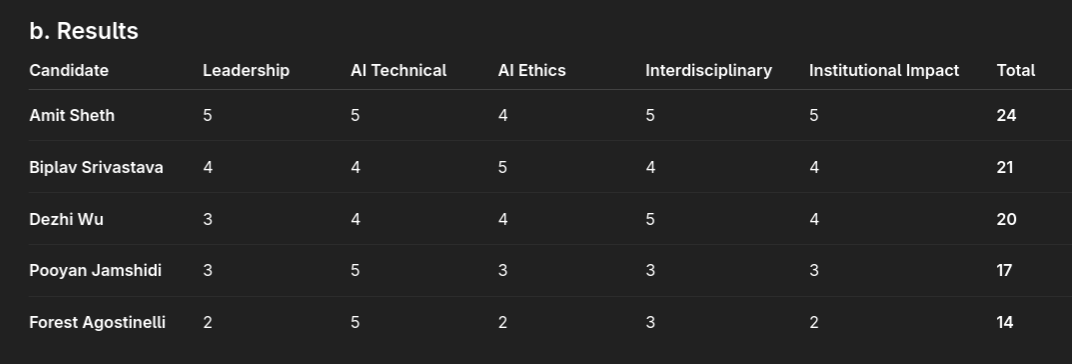
\includegraphics[width=1\textwidth]{results.png}
    \caption{The output of ChatGPT 5}
\end{figure}

\section{Conclusion}

The LLM chose Amit Sheth to hire for the position, scoring him a 24 out of 25.
The guy already has a leadership role for AI at the university, so this fits pretty
well onto reality in my opinion.

The ethical considerations here are that the decision was made exclusively AI, so this decision
may not necessarily reflect the context in which this hire is being made, and that it hasn't met any of these
people on a personal level.

Some decent part of this methodology is that the decision was made without the AI knowing the race, gender, 
age etc of the candidates so that can't factor in unfairly as easily if those factors were included. 
The ramifications of making a bad choice could be funds what weren't used well, a bad candidate being 
hired, or damaging of trust if it gets out that AI was used to make the decision. 

\end{document}
